This appendix reports supplementary determinants, heterogeneity, and ancillary consequence tests referenced in the main text. Tables~\ref{tab:appendix_det_reduced}, \ref{tab:appendix_det_full}, and~\ref{tab:appendix_det_intensity} report determinant specifications; Table~\ref{tab:appendix_size_heterogeneity} reports size heterogeneity in market outcomes; Tables~\ref{tab:appendix_issue_window_market}--\ref{tab:appendix_matched_ai_talking} report supporting market and matching checks; and Figure~\ref{fig:appendix_chatgpt_eventstudy} reports the supporting post-ChatGPT event-study path.

\begin{table}[H]
\centering
\caption{Reduced-baseline determinants of PatentMismatch}
\label{tab:appendix_det_reduced}
\small
\resizebox{\textwidth}{!}{%
\begin{tabular}{>{\raggedright\arraybackslash}p{0.34\textwidth}cccccc}
\hline
Variable & \multicolumn{6}{c}{Dependent variable: any PatentMismatch incident, 2016--2025} \\
 & Log assets & Cash/assets & Leverage & CAPX/assets & ROA & Multivar. \\
 & (1) & (2) & (3) & (4) & (5) & (6) \\
\hline
Log assets & 0.012*** &  &  &  &  & 0.012*** \\
 & (0.004) &  &  &  &  & (0.004) \\
Cash/assets &  & -0.024 &  &  &  & 0.033 \\
 &  & (0.034) &  &  &  & (0.033) \\
Leverage &  &  & 0.041 &  &  & 0.028 \\
 &  &  & (0.036) &  &  & (0.037) \\
CAPX/assets &  &  &  & 0.016 &  & -0.008 \\
 &  &  &  & (0.263) &  & (0.281) \\
ROA &  &  &  &  & 0.013 & 0.001 \\
 &  &  &  &  & (0.009) & (0.009) \\
Industry FE & Y & Y & Y & Y & Y & Y \\
All baseline covars. & N & N & N & N & N & Y \\
Baseline year & 2016 & 2016 & 2016 & 2016 & 2016 & 2016 \\
Adj. $R^2$ & 0.287 & 0.283 & 0.283 & 0.285 & 0.285 & 0.287 \\
Observations & 2,680 & 2,680 & 2,666 & 2,666 & 2,676 & 2,652 \\
\hline
\end{tabular}%
}
\caption*{\footnotesize \textit{Note.} This table revisits the firm-level PatentMismatch determinants specification using the reduced baseline characteristic set. The dependent variable is an indicator for whether the firm records at least one PatentMismatch incident during the period 2016--2025. Baseline characteristics are measured in 2016 and include log assets, cash/assets, leverage, CAPX/assets, and ROA. This reduced specification preserves sample size relative to the fuller baseline set. *, **, and *** denote significance at the 10\%, 5\%, and 1\% level, respectively.}
\end{table}


\begin{table}[H]
\centering
\caption{Full-baseline determinants of PatentMismatch}
\label{tab:appendix_det_full}
\small
\resizebox{\textwidth}{!}{%
\begin{tabular}{>{\raggedright\arraybackslash}p{0.34\textwidth}cccccccc}
\hline
Variable & \multicolumn{8}{c}{Dependent variable: any PatentMismatch incident, 2016--2025} \\
 & Log assets & Cash/assets & Leverage & R\&D/assets & CAPX/assets & ROA & Employees (k) & Multivar. \\
 & (1) & (2) & (3) & (4) & (5) & (6) & (7) & (8) \\
\hline
Log assets & 0.012*** &  &  &  &  &  &  & 0.009** \\
 & (0.004) &  &  &  &  &  &  & (0.003) \\
Cash/assets &  & -0.024 &  &  &  &  &  & 0.037 \\
 &  & (0.034) &  &  &  &  &  & (0.046) \\
Leverage &  &  & 0.041 &  &  &  &  & 0.028 \\
 &  &  & (0.036) &  &  &  &  & (0.059) \\
R\&D/assets &  &  &  & -0.029 &  &  &  & -0.025 \\
 &  &  &  & (0.033) &  &  &  & (0.050) \\
CAPX/assets &  &  &  &  & 0.016 &  &  & -0.497 \\
 &  &  &  &  & (0.263) &  &  & (0.376) \\
ROA &  &  &  &  &  & 0.013 &  & -0.001 \\
 &  &  &  &  &  & (0.009) &  & (0.017) \\
Employees (k) &  &  &  &  &  &  & 0.000 & 0.000 \\
 &  &  &  &  &  &  & (0.000) & (0.000) \\
Industry FE & Y & Y & Y & Y & Y & Y & Y & Y \\
All baseline covars. & N & N & N & N & N & N & N & Y \\
Baseline year & 2016 & 2016 & 2016 & 2016 & 2016 & 2016 & 2016 & 2016 \\
Adj. $R^2$ & 0.287 & 0.283 & 0.283 & 0.132 & 0.285 & 0.285 & 0.278 & 0.133 \\
Observations & 2,680 & 2,680 & 2,666 & 1,466 & 2,666 & 2,676 & 2,479 & 1,331 \\
\hline
\end{tabular}%
}
\caption*{\footnotesize \textit{Note.} This table presents the fuller cross-sectional determinants specification for whether a firm records at least one PatentMismatch incident during the period 2016--2025. Baseline characteristics are measured in 2016 and include log assets, cash/assets, leverage, R\&D/assets, CAPX/assets, ROA, and the number of employees. *, **, and *** denote significance at the 10\%, 5\%, and 1\% level, respectively.}
\end{table}


\begin{table}[H]
\centering
\caption{Full-baseline determinants of PatentMismatch intensity}
\label{tab:appendix_det_intensity}
\small
\resizebox{\textwidth}{!}{%
\begin{tabular}{>{\raggedright\arraybackslash}p{0.34\textwidth}cccccccc}
\hline
Variable & \multicolumn{8}{c}{Dependent variable: PatentMismatch share among AI-talking years, 2016--2025} \\
 & Log assets & Cash/assets & Leverage & R\&D/assets & CAPX/assets & ROA & Employees (k) & Multivar. \\
 & (1) & (2) & (3) & (4) & (5) & (6) & (7) & (8) \\
\hline
Log assets & 0.004 &  &  &  &  &  &  & -0.006 \\
 & (0.004) &  &  &  &  &  &  & (0.005) \\
Cash/assets &  & -0.073* &  &  &  &  &  & -0.045 \\
 &  & (0.042) &  &  &  &  &  & (0.052) \\
Leverage &  &  & 0.060 &  &  &  &  & 0.042 \\
 &  &  & (0.039) &  &  &  &  & (0.073) \\
R\&D/assets &  &  &  & -0.042* &  &  &  & -0.078 \\
 &  &  &  & (0.023) &  &  &  & (0.050) \\
CAPX/assets &  &  &  &  & -0.031 &  &  & -0.434* \\
 &  &  &  &  & (0.165) &  &  & (0.250) \\
ROA &  &  &  &  &  & 0.011* &  & 0.002 \\
 &  &  &  &  &  & (0.007) &  & (0.013) \\
Employees (k) &  &  &  &  &  &  & 0.000 & -0.000 \\
 &  &  &  &  &  &  & (0.000) & (0.000) \\
Industry FE & Y & Y & Y & Y & Y & Y & Y & Y \\
All baseline covars. & N & N & N & N & N & N & N & Y \\
Baseline year & 2016 & 2016 & 2016 & 2016 & 2016 & 2016 & 2016 & 2016 \\
Adj. $R^2$ & 0.271 & 0.272 & 0.271 & 0.141 & 0.272 & 0.272 & 0.265 & 0.135 \\
Observations & 2,680 & 2,680 & 2,666 & 1,466 & 2,666 & 2,676 & 2,479 & 1,331 \\
\hline
\end{tabular}%
}
\caption*{\footnotesize \textit{Note.} This companion table uses the share of AI-talking years flagged as PatentMismatch during the period 2016--2025 as the dependent variable rather than the extensive-margin indicator. The baseline characteristics are measured in 2016 and correspond to the full baseline set. *, **, and *** denote significance at the 10\%, 5\%, and 1\% level, respectively.}
\end{table}


\begin{table}[!htbp]
\centering
\footnotesize
\caption{Size heterogeneity in filing-date and post-filing mismatch effects}
\label{tab:appendix_size_heterogeneity}
\begin{tabular}{llccc}
\hline
  && Small subsample & Big subsample & Pooled interaction \\
\hline
 \multicolumn{5}{l}{\textit{Panel A. Dependent variable: CAR[-1,+1]}}\\
 &PatentMismatch & 0.0013 (0.0065) & 0.0014 (0.0044) & 0.0011 (0.0041) \\
 &PatentMismatch × Small &  &  & 0.0033 (0.0059) \\
 &Implied mismatch effect, small firms &  &  & 0.0043 (0.0055) \\
 &Small &  &  & -0.0036 (0.0043) \\
 &AS ratio & -0.0039 (0.0046) & 0.0050 (0.0040) & 0.0018 (0.0030) \\
 &AI Focus & 0.0032 (0.0033) & -0.0042 (0.0026) & -0.0010 (0.0020) \\
 &Controls & Y & Y & Y \\
 &Industry FE & Y & Y & Y \\
 &Filing-year FE & Y & Y & Y \\
 &Observations & 3,556& 3,571& 7,127\\
 &Adj. $R^2$ & 0.024 & 0.003 & 0.013 \\
 \multicolumn{5}{l}{\textit{Panel B. Dependent variable: BHAR[+2,+63]}}\\
 &PatentMismatch & 0.0102 (0.0231) & -0.0055 (0.0133) & -0.0049 (0.0123) \\
 &PatentMismatch × Small &  &  & 0.0171 (0.0191) \\
 &Implied mismatch effect, small firms &  &  & 0.0122 (0.0189) \\
 &Small &  &  & -0.0188 (0.0121) \\
 &AS ratio & 0.0049 (0.0166) & 0.0066 (0.0090) & 0.0059 (0.0086) \\
 &AI Focus & -0.0037 (0.0114) & -0.0053 (0.0064) & -0.0042 (0.0059) \\
 &Controls & Y & Y & Y \\
 &Industry FE & Y & Y & Y \\
 &Filing-year FE & Y & Y & Y \\
 &Observations & 3,435& 3,473& 6,908\\
 &Adj. $R^2$ & 0.024 & 0.033 & 0.025 \\
\hline
\end{tabular}
\caption*{\footnotesize \textit{Note.} This table reports heterogeneity in the filing-date and post-filing pricing effects by firm size. Small firms are defined using the monthly active-sample median lagged market capitalization from CRSP. The table is included as supporting evidence because the cleaner return and valuation patterns are concentrated outside the largest firms.}
\end{table}


\begin{table}[p]
\centering
\scriptsize
\setlength{\tabcolsep}{2pt}
\caption{Market reactions in capital-raising windows}
\label{tab:appendix_issue_window_market}
\resizebox{\textwidth}{!}{%
\begin{tabular}{llccccrrr}
\hline
Panel & Outcome & PM $\times$ Issue & LowCred. $\times$ Issue & AppMismatch $\times$ Issue & Baseline PM & IssueWindow & Mean & Obs. \\
\hline
\multicolumn{9}{l}{\textit{Panel A. Filing-year market reactions in all issue-eligible firms}} \\
 & CAR[-1,+1] & 0.0058 (0.0089) & 0.0074 (0.0085) & 0.0046 (0.0088) & -0.0009 (0.0039) & -0.0055 (0.0055) & 0.000 & 4,378 \\
 & BHAR[+2,+63] & 0.0716** (0.0346) & 0.0577* (0.0313) & 0.0526 (0.0341) & -0.0272*** (0.0095) & 0.0279 (0.0174) & -0.029 & 4,376 \\
 & BHAR[+2,+252] & 0.3885 (0.2433) & 0.2496 (0.1922) & 0.3498 (0.2353) & 0.0094 (0.0242) & 0.1729*** (0.0548) & -0.024 & 4,360 \\
\multicolumn{9}{l}{\textit{Panel B. Filing-year market reactions in non-big firms}} \\
 & CAR[-1,+1] & 0.0090 (0.0136) & 0.0163 (0.0134) & 0.0095 (0.0134) & -0.0014 (0.0080) & -0.0054 (0.0086) & -0.008 & 2,024 \\
 & BHAR[+2,+63] & 0.0918* (0.0504) & 0.1139** (0.0456) & 0.0823* (0.0487) & -0.0353** (0.0176) & 0.0282 (0.0241) & -0.068 & 2,023 \\
 & BHAR[+2,+252] & 0.4976 (0.3488) & 0.3805 (0.2888) & 0.4766 (0.3324) & 0.0398 (0.0427) & 0.1883** (0.0747) & -0.119 & 2,009 \\
\hline
\end{tabular}%
}
\caption*{\footnotesize \textit{Note.} This table reports filing-year return regressions that interact low-credibility AI disclosure measures with the capital-raising window used in Table~\ref{tab:capital_raising_timing_v32}. IssueWindow equals one when next-year CRSP shares outstanding growth exceeds 5\%. The three interaction columns report coefficients for the interaction between the listed disclosure measure and IssueWindow. Baseline PM is the PatentMismatch coefficient outside issue windows, and IssueWindow is the level effect in the canonical PatentMismatch specification. Return outcomes are in decimal units. All regressions include filing-year fixed effects, annual controls, and firm-clustered standard errors. *, **, and *** denote significance at the 10\%, 5\%, and 1\% level, respectively.}
\end{table}


\begin{table}[p]
\centering
\small
\caption{Predictive post-filing return regressions with richer controls}
\label{tab:appendix_predictive_return_controls}
\resizebox{\textwidth}{!}{%
\begin{tabular}{lcccc}
\hline
 & Core controls & + operating controls & + market characteristics & + market + patent history \\
 & (1) & (2) & (3) & (4) \\
\hline
\multicolumn{5}{l}{\textit{Panel A. Dependent variable: BHAR[+2,+63]}} \\
PatentMismatch & 0.0005 (0.0099) & 0.0058 (0.0124) & 0.0086 (0.0110) & 0.0065 (0.0117) \\
AS ratio & 0.0021 (0.0073) & 0.0076 (0.0088) & 0.0115 (0.0079) & 0.0104 (0.0081) \\
AI Focus & -0.0044 (0.0053) & -0.0050 (0.0059) & -0.0072 (0.0056) & -0.0063 (0.0059) \\
Outcome mean & -0.0445 & -0.0448 & -0.0474 & -0.0474 \\
Observations & 6,958 & 4,243 & 4,113 & 4,113 \\
Adj. $R^2$ & 0.043 & 0.064 & 0.227 & 0.227 \\
\multicolumn{5}{l}{\textit{Panel B. Dependent variable: BHAR[+2,+252]}} \\
PatentMismatch & 0.0216 (0.0266) & 0.0206 (0.0319) & 0.0322 (0.0224) & 0.0365 (0.0234) \\
AS ratio & -0.0226 (0.0183) & -0.0065 (0.0213) & 0.0090 (0.0154) & 0.0115 (0.0158) \\
AI Focus & 0.0151 (0.0136) & 0.0167 (0.0154) & 0.0012 (0.0106) & -0.0007 (0.0108) \\
Outcome mean & -0.0807 & -0.0569 & -0.0569 & -0.0569 \\
Observations & 4,644 & 2,936 & 2,936 & 2,936 \\
Adj. $R^2$ & 0.114 & 0.156 & 0.536 & 0.536 \\
\hline
\end{tabular}%
}
\caption*{\footnotesize \textit{Note.} This table asks whether post-filing return relations are absorbed by richer observable controls. The unit is an AI-talking annual filing event. Core controls include log assets, leverage, cash/assets, and ROA. Operating controls add R\&D/assets, CAPX/assets, and sales growth. Market characteristics add lagged market capitalization, annual return, annual buy-and-hold abnormal return, volatility, and market age. Patent history adds lagged AI patenting. All specifications include SIC2 and filing-year fixed effects, and standard errors are clustered by firm.}
\end{table}


\begin{table}[p]
\centering
\small
\caption{Matched AI-talking comparison sample}
\label{tab:appendix_matched_ai_talking}
\begin{tabular}{lccccc}
\hline
Outcome & Treated mean & Control mean & Difference & $p$-value & Matched pairs \\
\hline
CAR[-1,+1] & 0.0016 & 0.0006 & 0.0010 & 0.812 & 1,294 \\
BHAR[+2,+21] & -0.0307 & -0.0258 & -0.0049 & 0.484 & 1,270 \\
BHAR[+2,+63] & -0.0513 & -0.0477 & -0.0036 & 0.755 & 1,213 \\
BHAR[+2,+126] & -0.0715 & -0.0814 & 0.0099 & 0.564 & 1,121 \\
BHAR[+2,+252] & -0.0648 & -0.0840 & 0.0191 & 0.523 & 692 \\
\hline
\end{tabular}
\caption*{\footnotesize \textit{Note.} This table compares PatentMismatch filing events with matched AI-talking filing events that are not flagged as PatentMismatch. AI-talking events are filings with at least one AI-related sentence. Matches are exact on filing year and SIC2 industry and nearest on lagged market capitalization, lagged annual BHAR, lagged annual return, log assets, leverage, cash/assets, and ROA, subject to a standardized-distance caliper of 1.50. The matched sample contains 1,297 pairs, with a median match distance of 0.857 and a maximum absolute matched standardized mean difference of 0.025 across the matching covariates. Return outcomes are in decimal units.}
\end{table}


\begin{figure}[p]
\centering
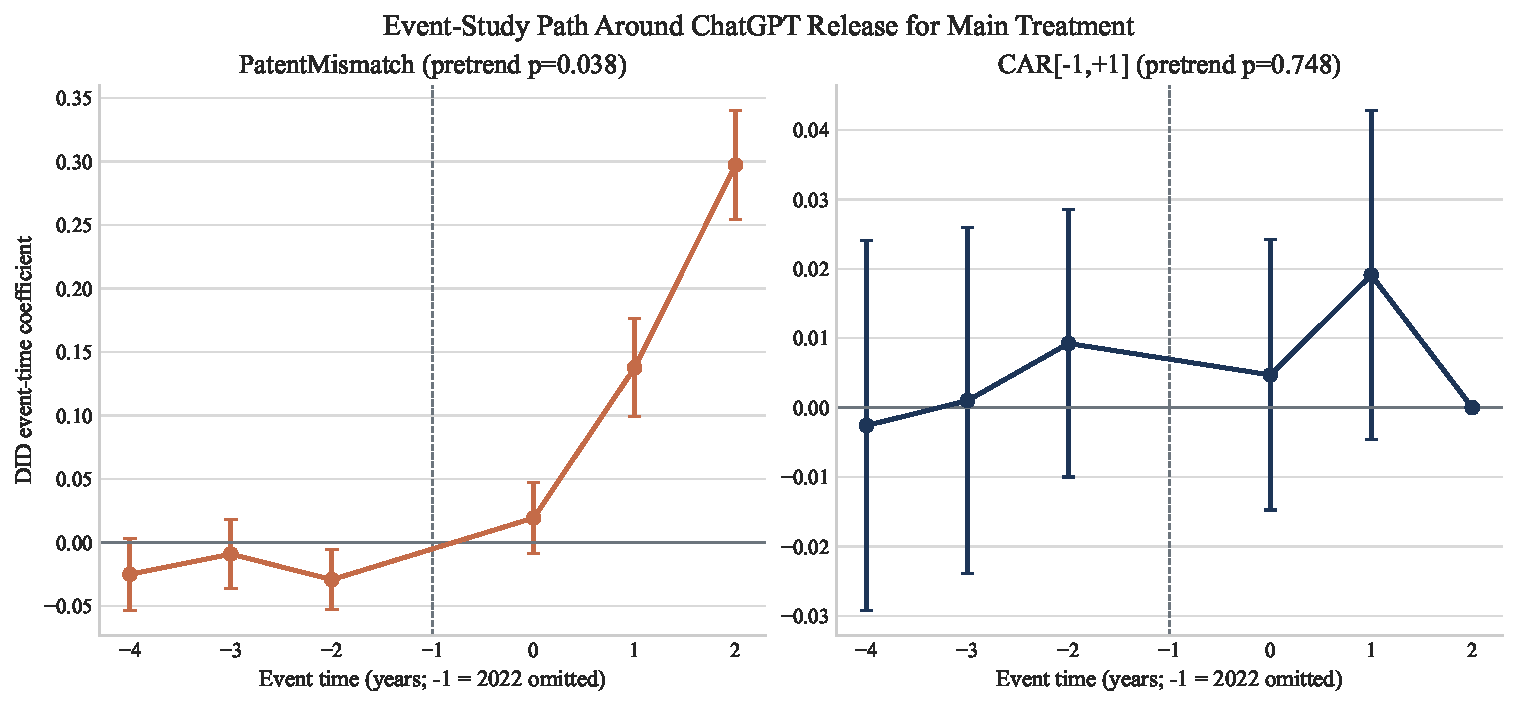
\includegraphics[width=\textwidth]{figures/figureC1.pdf}
\caption{Event-study path around the release of ChatGPT}
\label{fig:appendix_chatgpt_eventstudy}
\caption*{\footnotesize \textit{Note.} This figure plots event-time coefficients for the baseline post-ChatGPT treatment around late 2022. The left panel reports PatentMismatch and the right panel reports filing-date CAR[$-1,+1$]. The figure is included as supporting evidence for the post-2022 disclosure-composition patterns and reports pretrend diagnostics to aid interpretation.}
\end{figure}
